 \documentclass{article}

\usepackage{graphicx} % Allows including images
\usepackage{stackengine}
\usepackage{scalerel}
\usepackage{xcolor}
\usepackage{geometry}
\usepackage{multicol}
\usepackage{listings}

\graphicspath{{./../img/}}
\renewcommand{\abstractname}{}
\renewcommand{\tt}[1]{\texttt{#1}}

\newcommand\dangersign[1][2ex]{%
  \renewcommand\stacktype{L}%
  \scaleto{\stackon[1.3pt]{\color{red}$\triangle$}{\tiny !}}{#1}%
}

\newcommand{\warn}[1]{\begin{center}
\begin{tabular}{ c  p{12cm} }
\dangersign[22pt] & \vspace{-0.6cm} #1
\end{tabular}
\end{center}}

\geometry{
 a4paper,
 left=30mm,
 right=30mm,
 top=30mm,
 bottom=30mm
 }

\lstset{language=Python,
		commentstyle=\color{gray},
		keywordstyle=\color{blue},
		numberstyle=\color{yellow},
		stringstyle=\color{purple}
}


\title{\texttt{theia} \\ \quad \\A 3D Gaussian beam tracer \\ \quad \\ Version 0.1.0 \\ \textit{API Guide}}

\author{Rapha\"el Duque}

\begin{document}

\maketitle
\begin{abstract}
theia is a command line program and Python library for 3D Gaussian beam tracing. It supports many different types of optical components, general 3D placing and orientation of these components and general astigmatic Gaussian beams, among other features. theia was developed at the Optics Group of the Virgo gravitational observatory in Cascina, Italy. Please see the \tt{README.md} file of \tt{theia} or surf to \tt{http://37.117.61.221:56000} for more information.

This document is an Application Programming Interface Guide for the theia library. It give somewhat more detail on the algorithm and data structures of theia and how they are implemented in theia. This guide may be useful to anyone who wants to use theia to develop their own optical simulation scripts, and to anyone who would like to contribute to theia.

Throughout this document, Unix \tt{paths/like/this} are understood as relative to the theia project root directory (\textit{e.g.} \tt{doc/img/flow.png}) and Python import statements \tt{like.this.one} are understood as relative the theia package root directory (\textit{e.g.} \tt{running.simulation.Simulation.\_\_init\_\_}).
\end{abstract}

\tableofcontents
\newpage

\subsection{A note on global variables}
The theia CLI tool uses a certain number of global variables in order to keep values which don't change along the execution. These global variables are consequently needed by a certain number of functions defined in the library in order for the CLI tool to be as functional as possible. When using theia as a library, one may not need all these globals and they may even get in the way of development.

\paragraph{How to take care of the globals once and for all.}The global variables are \textit{all} declared in \tt{helpers.settings} and are initialized with \tt{helpers.settings.init} at the very beginning of \tt{main.main}, which takes in a dictionary and reads the globals from there. If you don't want to hear about the globals, you can place the following snippet (found in \tt{tests/test\_simulation.py}) at the beginning of your script and not worry about the globals.

\begin{lstlisting}
# use this snippet and all globals worries are gone
from theia.helpers.settings import init

# initialize globals in a dictionary
dic = {'info': False, 'warning': False, 'text': False, 'cad': False,
		'fname': 'test_optics'}

init(dic)

# you're all set 
\end{lstlisting}

\paragraph{Who uses the globals?}Here is a table listing the global variables and which functions use them.

\begin{table}[h]
\begin{center}

\begin{tabular}{|c | l |}
\hline
\textbf{Global} & \textbf{Used by} \\ \hline \hline

\tt{info} & \tt{optics.beamdump.BeamDump.hit} \\
& \tt{optics.lens.Lens.hitActive} \\
& \tt{optics.mirror.Mirror.hitHR} \\
& \tt{optics.mirror.Mirror.hitAR} \\
& \tt{optics.optic.Optic.hitSide} \\
& \tt{tree.beamtree.treeOfBeam} \\ \hline

\tt{warning} & \tt{optic.mirror.Mirror.\_\_init\_\_} \\
& \tt{optic.thicklens.ThickLens.\_\_init\_\_} \\
& \tt{optic.thinlens.ThinLens.\_\_init\_\_} \\
& \tt{running.simulation.Simulation.run} \\ \hline

\tt{text, cad, fname} & \tt{main.main} \\ \hline

\end{tabular}
\caption{The global variables of theia and the functions who use them}
\label{globals}
\end{center}
\end{table}
\subsection{Classes and inheritance hierarchy}
Figure \ref{inheritancehierarchy} presents the inheritance hierarchy of the classes of theia. If you see a method twice, it just means the daughter class reimplements the method.

\begin{figure}[h]
\begin{center}
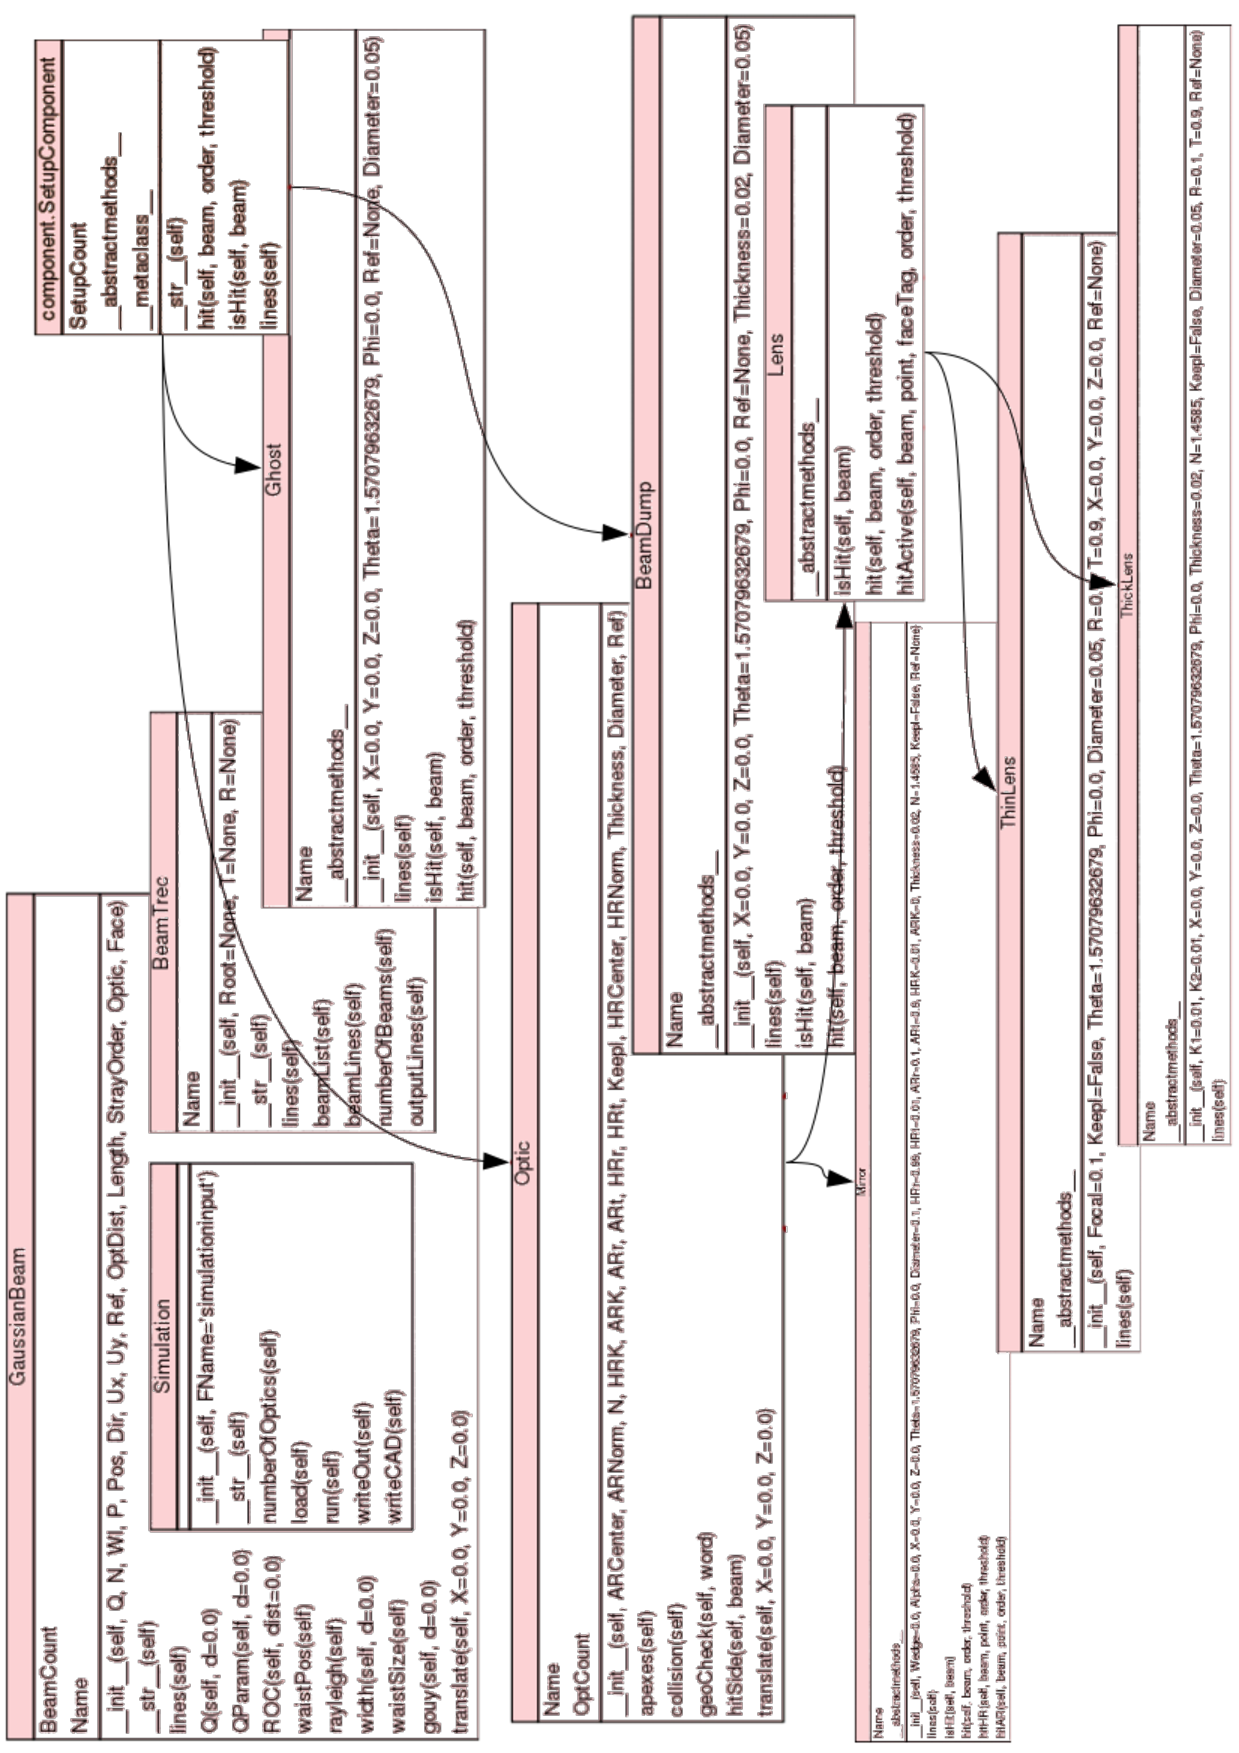
\includegraphics[scale=1]{inheritancehierarchy}
\label{inheritancehierarchy}
\end{center}
\end{figure}
\paragraph{A word on initializer default values.}We try to avoid surprises and stay consistent throughout the code with the following policies concerning classes at the leaves of the inheritance graph:

\begin{enumerate}
\item For classes whose initializers will be called only with input form users (read from an input file or in a a script), \textit{every} parameter of the constructor has a default value and the constructor can be called \textit{without arguments}. What's more, the input of the user is processed through the class initializer and then fed to the initializer of the mother class. For example, the user may provide \tt{X}, \tt{Y} and \tt{Z} to the constructor she or he calls, then these are processed and it is \tt{[X, Y, Z]} as a list (with types checked etc.) which is fed to the mother initializer. This concerns the constructors for \tt{ThinLens}, \tt{ThickLens}, \tt{Mirror}, \tt{BeamDump}.

\item For classes whose initializers are called solely internally, there are \textit{no default values}. These are the constructors of \tt{SetupComponent}, \tt{Optic}.

\item For classes that may be instantiated internally and by users, the class has a \tt{classmethod} decorated method, whose parameters \textit{all have default values} and which is intended to be used with input from the user, as the constructors described in the previous point 1. This method is named \tt{user\$CLASSNAME} and processes the input of the user into input for the class's proper \tt{\_\_init\_\_} initializer. On the other hand, this proper initializer is intended for internal use only and has \textit{no default values}. This is for example the case of the \tt{optics.beam.GaussianBeam} class, whose constructor is called internally to generate new beams and with user input read from the input file. In this last case it is \tt{userGaussianBeam} which is called.
\end{enumerate}

\paragraph{Abstract Base Classes.}The highest class of the optical classes hierarchy is the \tt{optics.component.SetupComponent} class. Its metaclass is set to \tt{abc.ABCMeta}, making it an abstract base class\footnote{See \tt{docs.python.org/2/library/abc.html} for details}. This essentially means that no daughter class of this class can be instantiated unless all the methods decorated with \tt{abc.abstractmethod} have been reimplemented by the daughter class. The methods concerned with this limitation are \tt{optics.component.SetupComponent.lines} and \tt{optics.component.SetupComponent.isHit}. Methods decorated with \tt{abstractmethod} in an abstract base class can eventually be implemented in the mother class, but in theia they all \tt{pass}, and could be called \textit{pure virtual} for someone coming from C++.
\subsection{Call graph}

Here is the call graph of the theia CLI tool, from which one can easily deduce the call graph of any individual function.


\begin{figure}[h]
\begin{center}
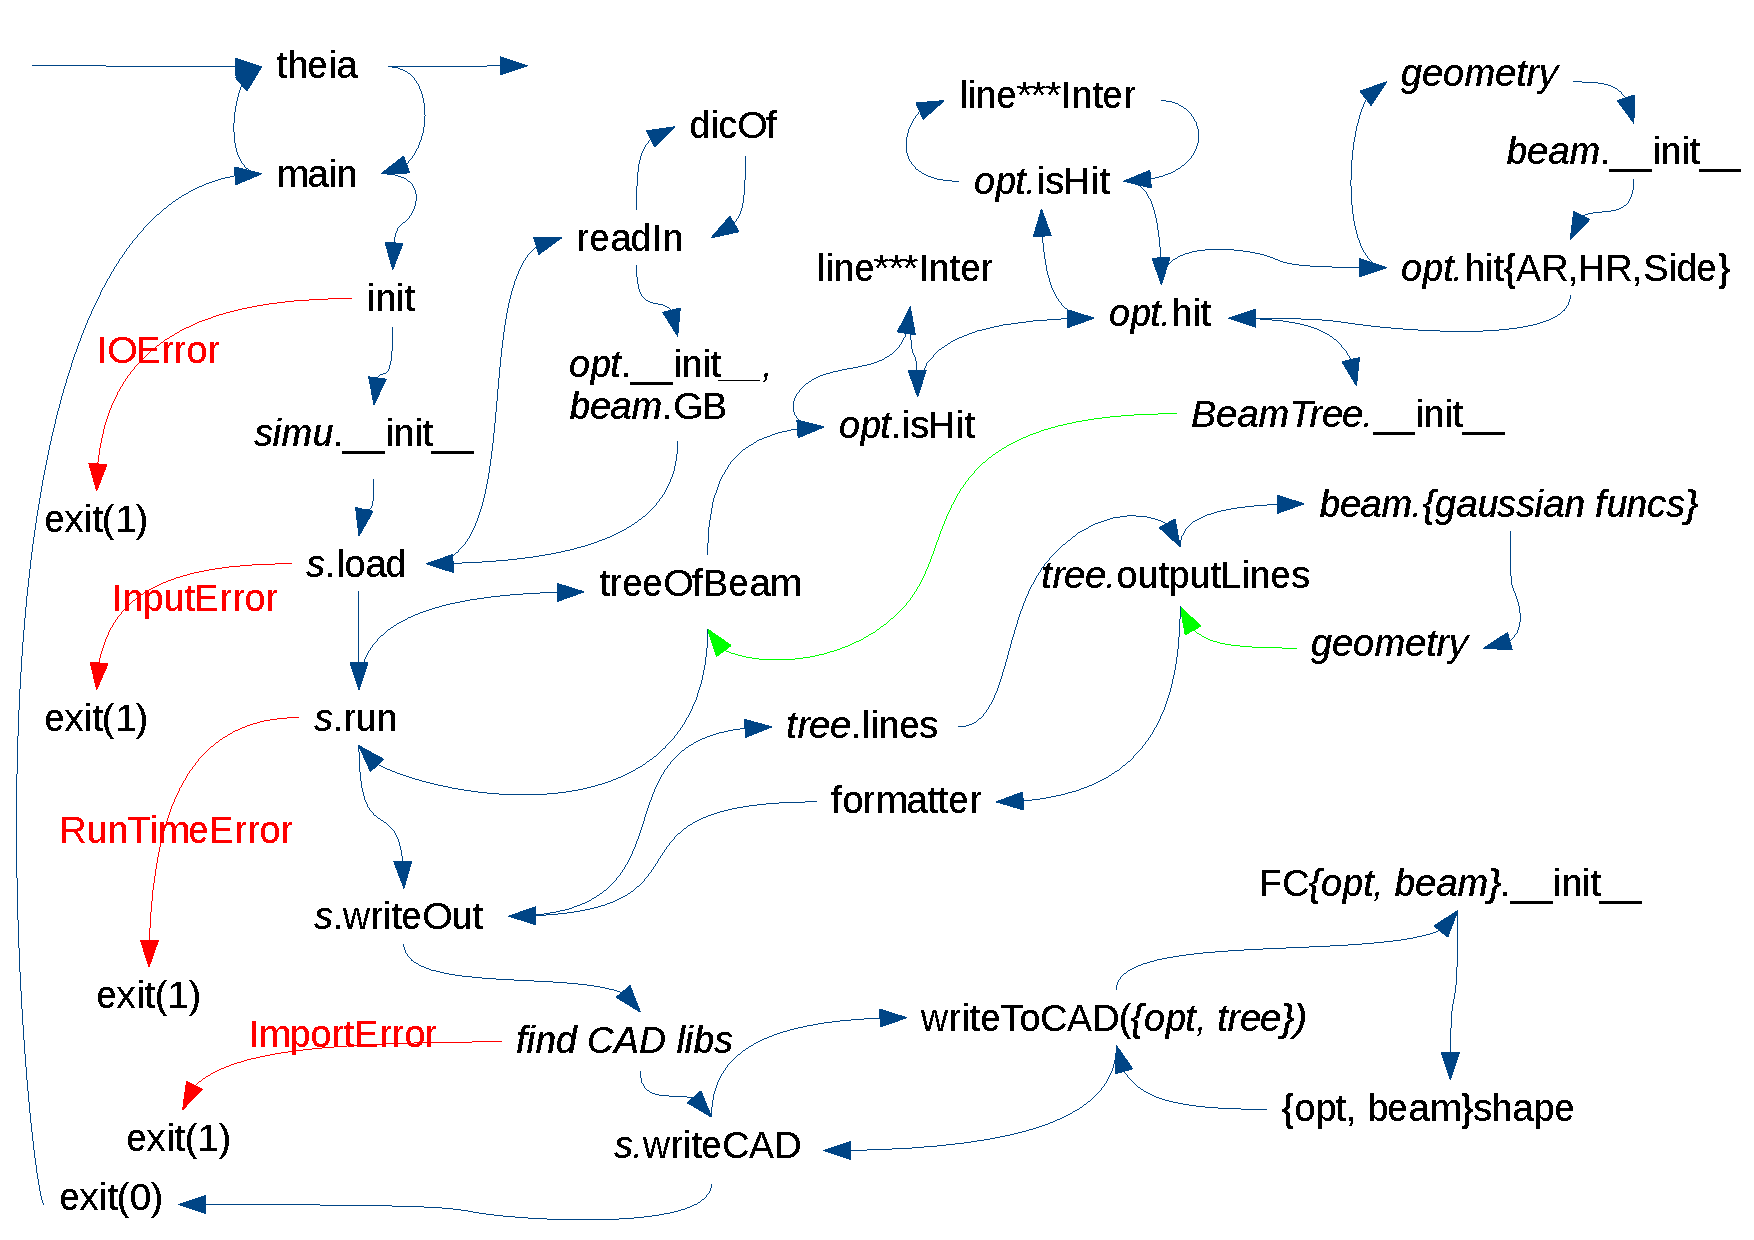
\includegraphics[scale=1]{callgraph}
\end{center}
\caption{Call graph of the theia CLI tool}
\label{callgraph}
\end{figure}

For a more concise view, here is the dependency tree of the functions of the theia library.

\begin{figure}[h]
\begin{center}
\includegraphics[scale=1]{functiondependencies}
\end{center}
\caption{Dependencies of the functions of the theia library}
\end{figure}

\paragraph{Note on the stack.}According to this call graph (figure \ref{callgraph}), the stack has a maximum height of $9~+~2(n-1)$ when there are $n$ levels of recursion. Generally, the program crashes -- if it crashes -- by recursion depth limit exceeding (leading to a handled \tt{RunTimeError} exception and an exit with an error code of 1) before causing a stack overflow.

\subsection{Miscellaneous remarks}

\paragraph{Coding style.}In the development of theia we have tried to stick to a couple of coding style conventions, which may help to review the code and are important to know for anyone wishing to contribute.

\begin{itemize}
\item The code of theia is heavily commented and doc-stringed, and it should stay that way in order for theia to be an accessible library.

\item Throughout the library, classes and attributes look \tt{LikeThis} whereas objects and methods look \tt{likeThis}.

\item There is an approximate (it isn't true only in the \tt{helpers} sub-package) \textit{one file} $\rightarrow$ \textit{one class} correspondence and files are named accordingly with the objects they define. Generally, we have a tendency to distribute functions in different modules if they provide different functionalities, regardless of the total number of modules. Functions are together in a module if they belong together, consequently they are many modules in theia.

\item We tend never to skip more than 1 line (Python is already very formatted).

\item \tt{\# Provides} lines at the very beginning of modules allow to know at a glance what variables, functions and classes the module provides.

\item Imports: import first from the Python standard library and third-party packages, then from theia sub-packages other than the current, then from the current theia sub-package. For theia sub-packages imports, always use the \tt{from ... import} idiom, always use relative imports (\tt{from ..helpers import interaction}) and for standard library and third-parties always \tt{import} before you \tt{from ... import}. We try to not import what we don't need.

\item Class doc-string: present class attributes before instance attributes and mention if they are inherited.
\end{itemize}

\paragraph{Writing to \tt{stdout} and files.}Many classes reimplement the \tt{\_\_str\_\_} method to have \tt{print(object)} print a neatly formated description of the object. To this effect there are two important methods: \tt{lines} (instance method) and \tt{helpers.tools.formatter} (global scope function). \tt{formatter} takes a list of strings (lines to output) and makes C-style indented output with curly braces in the right place in one large string. Basically, one has:

\begin{lstlisting}
# inside class scope
def __str__(self):
	return formatter(self.lines())
	
\end{lstlisting}
\end{document} 








































